\chapter{Introducción}\label{sec:intro}

\section{Introducción}

\subsection{Motivación y objetivos}
La electrónica digital forma parte de la rama de electrónica mas moderna y que evoluciona más rápidamente de la actualidad, debido a las ventajas de esta y las cuáles serán analizadas en el presente proyecto. Por ello, es importante llevar a todo el mundo esta tecnología, hacerla amigable y dotar a la sociedad de las herramientas necesarias para su correcto entendimiento, sin que ello suponga la realización de unos estudios superiores. \newline

Involucrarse de lleno en un proyecto tan poco desarrolado y con tan poco información, puede parecer un poco abrumador en principio, sobretodo cuando los problemas empiezan a aparecer, pero para cualquier ingeniero es todo un reto poder empezar a abrir camino sobre un campo determinado, ofreciendo a la sociedad algunas herramientas útiles para futuras implementaciones. \newline

Trabajar sobre una plataforma nativa de tu ciudad como es la IceZum Alhambra teniendo en cuenta el poco desarrollo en este campo, es además un honor que no hay que perder de vista a la hora de definir las motivaciones y objetivos. \newline

Electrónica digital, FPGAs, micro-controlador, lenguaje de descripción hardware, son sólo algunos de los conceptos más importantes sobre los que se sustentan el presente trabajo, y forma parte también de una de las más importantes líneas de investigación sobre ingenieros de todo el mundo. Es un objetivo poder llevar este concepto a las aulas de los más pequeños de la sociedad, haciendo uso para ello de librerías de bloques de implementación hardware que ayudarán en los sucesivos trabajos y abriendo el concepto de "robótica educativa".

\subsection{Planificación (Diagrama de Gantt)}

\begin{center}
	\begin{figure}[H]
		\center
		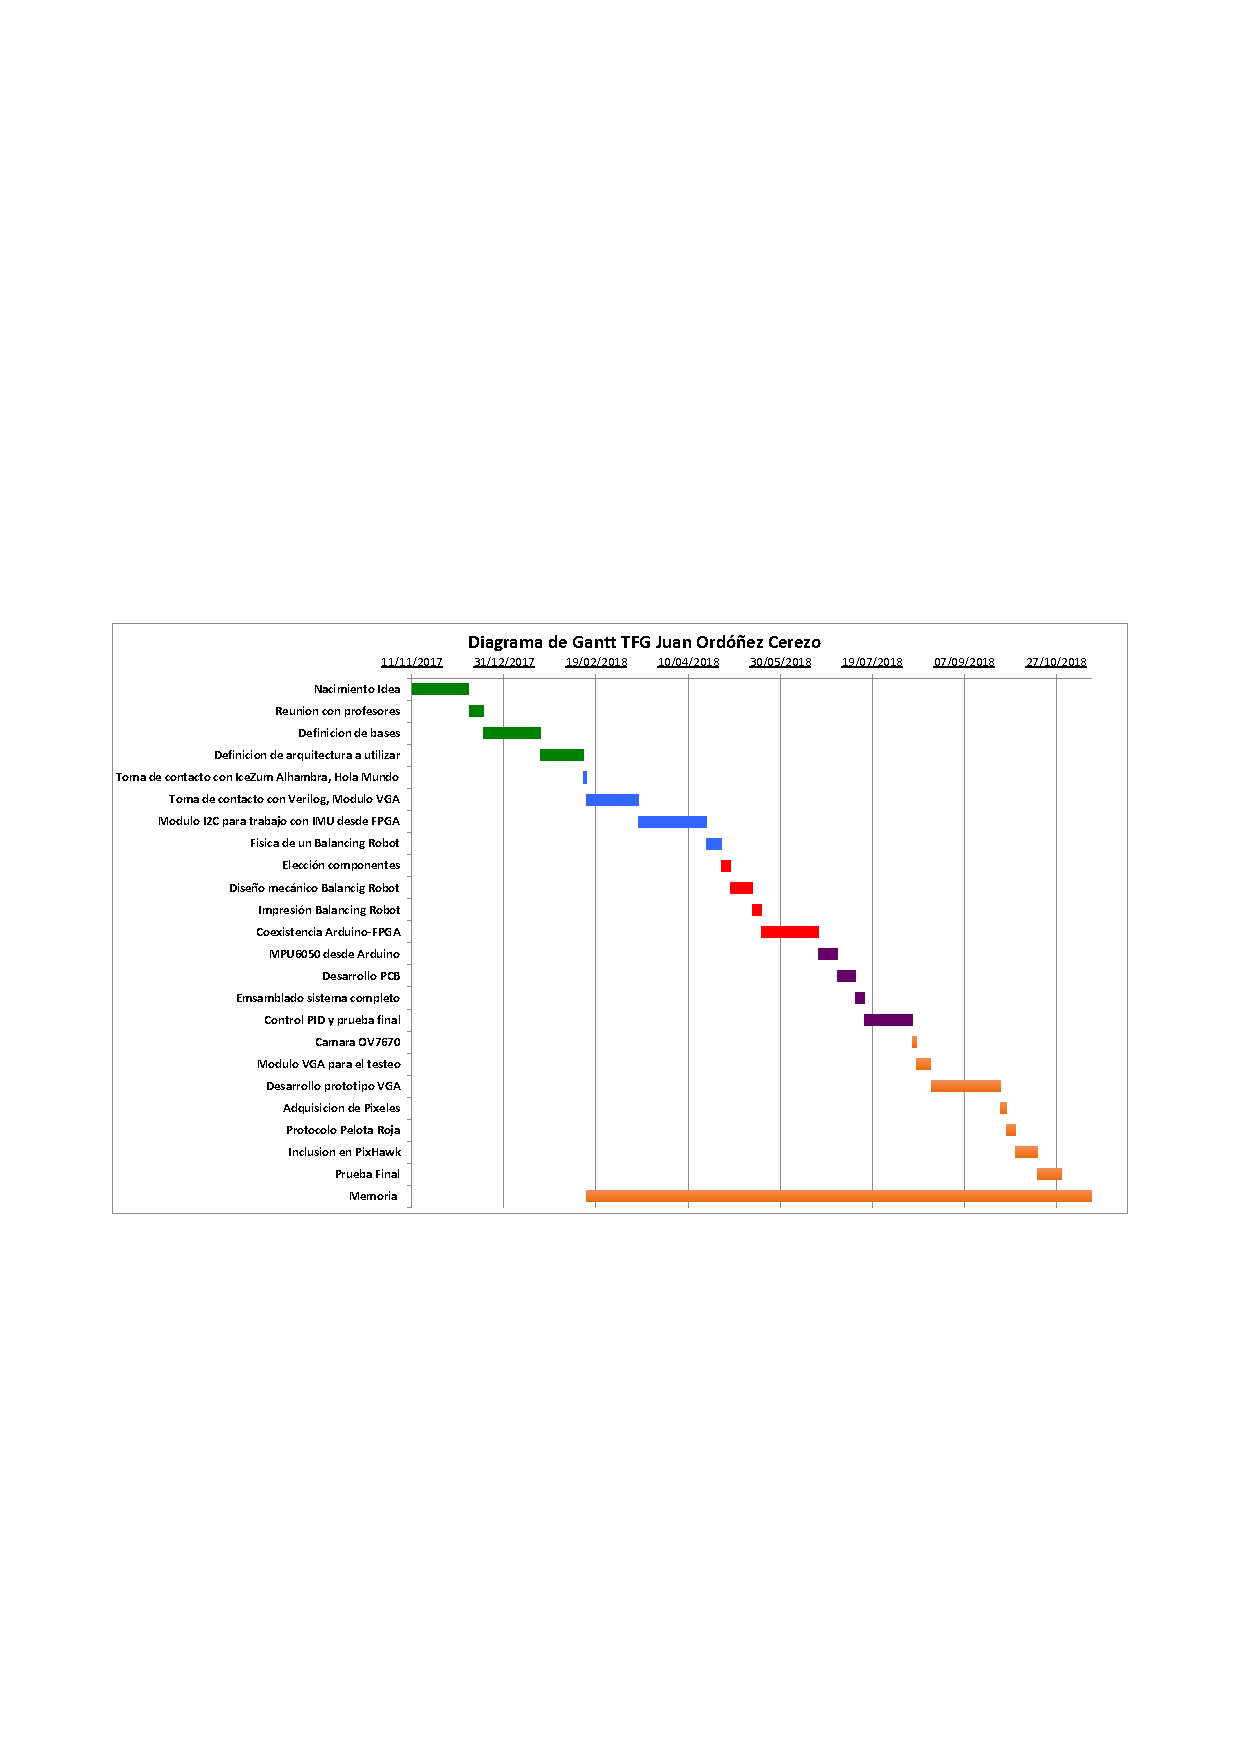
\includegraphics[trim = 15mm 85mm 0mm 100mm,clip, angle=-90, scale = 1.4]{imagenes/Introduction/Gantt.pdf}
		\label{fig:diagramaGantt}
	\end{figure}
\end{center}
\subsection{Metodología de trabajo}
Para introducir la metodología de trabajo seguida, se presenta la herramienta GitHub (figura \ref{fig:github}).\newline 

\begin{figure}[H]
	\center
	
\includegraphics[trim = 0mm 0mm 0mm 0mm, clip,scale=0.4]{imagenes/Introduction/github}
	\caption{Logo GitHub.}
	\label{fig:github}
\end{figure}


GitHub es una plataforma de desarrollo colaborativo de software para alojar proyectos utilizando el sistema de control de versiones Git. GitHub aloja tu proyecto en un repositorio y brinda herramientas muy útiles para el trabajo en equipo. \newline
Proporciona además la posibilidad de una Wiki para el mantenimiento de las versiones e información acerca de ellas. \newline
En el presente proyecto GitHub ha sido usado como un contenedor, donde se ha ido subiendo todo de manera parcial, normalmente, cuando se obtenía una versión estable sobre algunas de las ramas. \newline
De esta forma, y al ser abierto, cualquier persona ha podido seguir los avances de este, dudas, problemas, o incluso utilizar algunos de los módulos o material subidos. \newline
 
El proyecto puede encontrarse en la siguiente URL: \newline

\hyperref[]{https://github.com/RoboticsURJC-students/2017-tfg-juan-ordonez}

Un ejemplo de la trayectoria de este proyecto se representa en la captura de pantalla de GitHub en la figura \ref{fig:capturaGit}.

\begin{figure}[H]
	\center
	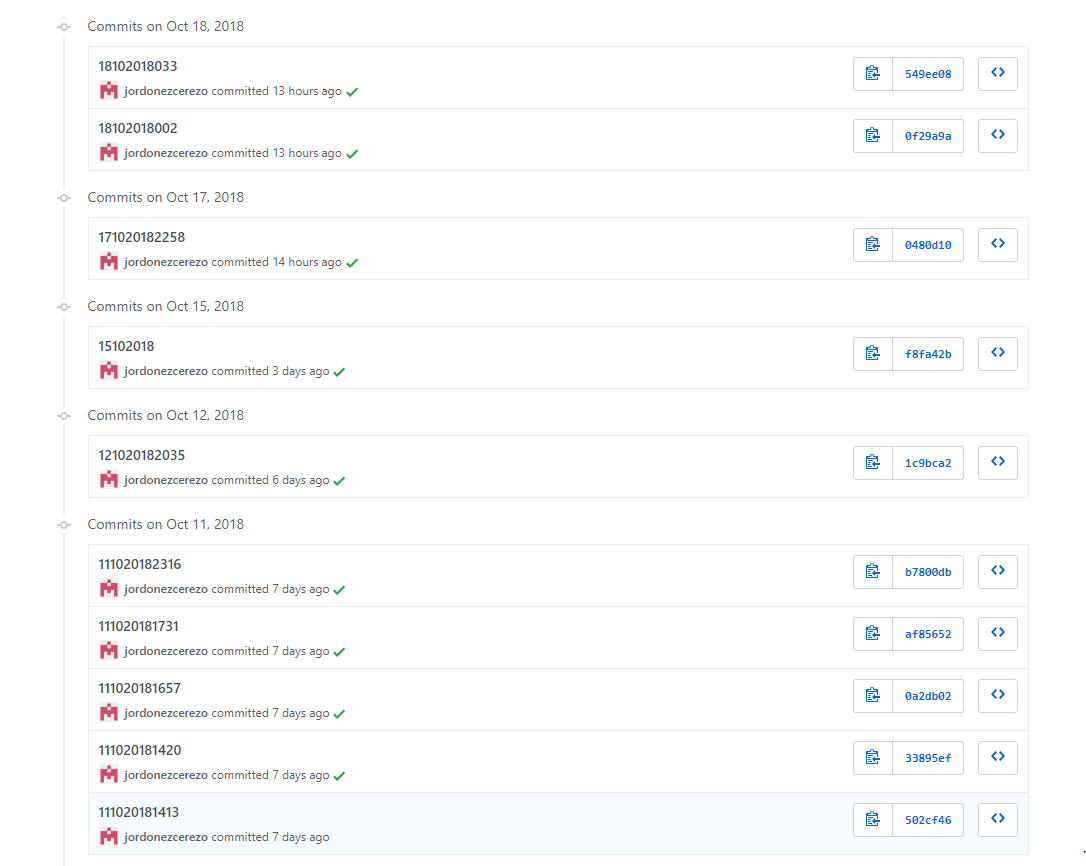
\includegraphics[trim = 0mm 0mm 0mm 0mm, clip,scale=0.5]{imagenes/Introduction/CapturaGit}
	\caption{Commits GitHub.}
	\label{fig:capturaGit}
\end{figure}

Para el buen cumplimiento de los objetivos planteados en primera instancia, y teniendo en cuenta la diferente localización de los componentes del trabajo, se hizo necesario el planteamiento de reuniones semanales (normalmente los Viernes) donde se pusiese en común lo trabajado durante la semana y se fijasen los siguientes objetivos. \newline

Para ello, se utilizo la herramienta se software libre llamada "Appear.in", la cuál ofrece videoconferencias entre varios usuarios al mismo instante (figura \ref{fig:appear}). 

\begin{figure}[H]
	\center
	
\includegraphics[trim = 0mm 0mm 0mm 0mm, clip,scale=0.3]{imagenes/Introduction/appear}
	\caption{Appear.in.}
	\label{fig:appear}
\end{figure}

\subsection{Estructura de la memoria}

La memoria está dividida en tres capítulos o partes diferenciadas. \newline
En la sección \ref{sec:Estado_arte} se explicará brevemente toda la parte teorica y conocimientos necesarios para el entendimiento del presente trabajo. Además se comentará la evolución hasta la actualidad de algunos sistemas propuestos.\newline

En la sección \ref{sec: BalancingRobot} se abordará en problema del Balancing Robot, y se diferenciara entre una parte de diseño y una parte de implementación, haciendo especial hincapié en el control PID que será utilizado en el capítulo siguiente. El Balancing Robot será capaz de mantenerse estable sobre dos ruedas horizontales.\newline

En la sección \ref{sec: Cuadricoptero} se abordará el problema de visión a bordo de un cuadricóptero. 
Una vez conseguidos los objetivos necesarios en la sección anterior, un cuadricoptero será capaz de seguir una pelota roja, por lo que se implementará el protocolo necesario para ello. \newline

Para terminar, en la sección \ref{sec: Conclusiones} se expondrán las conclusiones derivadas del trabajo completo, así como un posible trabajo futuro, errores a corregir, etc.   